% 依据固定候选 PDF 第 1 页重绘；source_id=src-71817304e261efb7deaf51c2a5f400421a95ac91a90313d8f558bee701a624f9
% PDF SHA-256: e5356797259eb22cc2b4f23019ad7ab044f282bdfc2a65df94dbbdcc502cfff5
% 保留原图边界、D 位于 AB、CD 实线以及 AO、OB、OC、OD 虚线关系；示意图不按比例。
\begin{center}
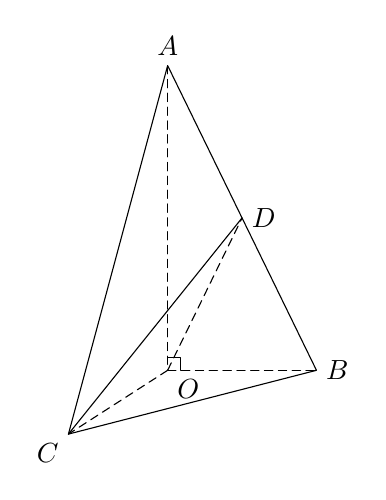
\begin{tikzpicture}[x=0.9cm,y=0.9cm,line join=round,line cap=round]
  \coordinate (A) at (0,4.3);
  \coordinate (O) at (0,0);
  \coordinate (B) at (2.1,0);
  \coordinate (C) at (-1.4,-0.9);
  \coordinate (D) at (1.05,2.15);
  \draw (A)--(C)--(B)--cycle;
  \draw (C)--(D);
  \draw[densely dashed] (A)--(O);
  \draw[densely dashed] (O)--(B);
  \draw[densely dashed] (O)--(C);
  \draw[densely dashed] (O)--(D);
  \draw (0.18,0)--(0.18,0.18)--(0,0.18);
  \node[above] at (A) {$A$};
  \node[right] at (B) {$B$};
  \node[below left] at (C) {$C$};
  \node[below right] at (O) {$O$};
  \node[right] at (D) {$D$};
\end{tikzpicture}
\end{center}
